%
% File: chap02.tex
%
\let\textcircled=\pgftextcircled
\chapter{Results}
\label{chap:result}

\initial{T}his chapter presents the results obtained during the experiment performed on September 14th, 2016. It presents the sample's half-life, its decay constant, and the analysis from the detector, allowing us to determine the isotopic composition.

\section{Sample activity}

The data, presented in appendix~\ref{app:app01}, is plotted on figure~\ref{fig:actsample}, along with its exponential least-square fit. One can appreciate the good fit obtained, with an $R^2$ value of 99.5\%, computed using equations~\ref{eq5} to~\ref{eq8}.

\begin{figure}[t!]
	\centering
	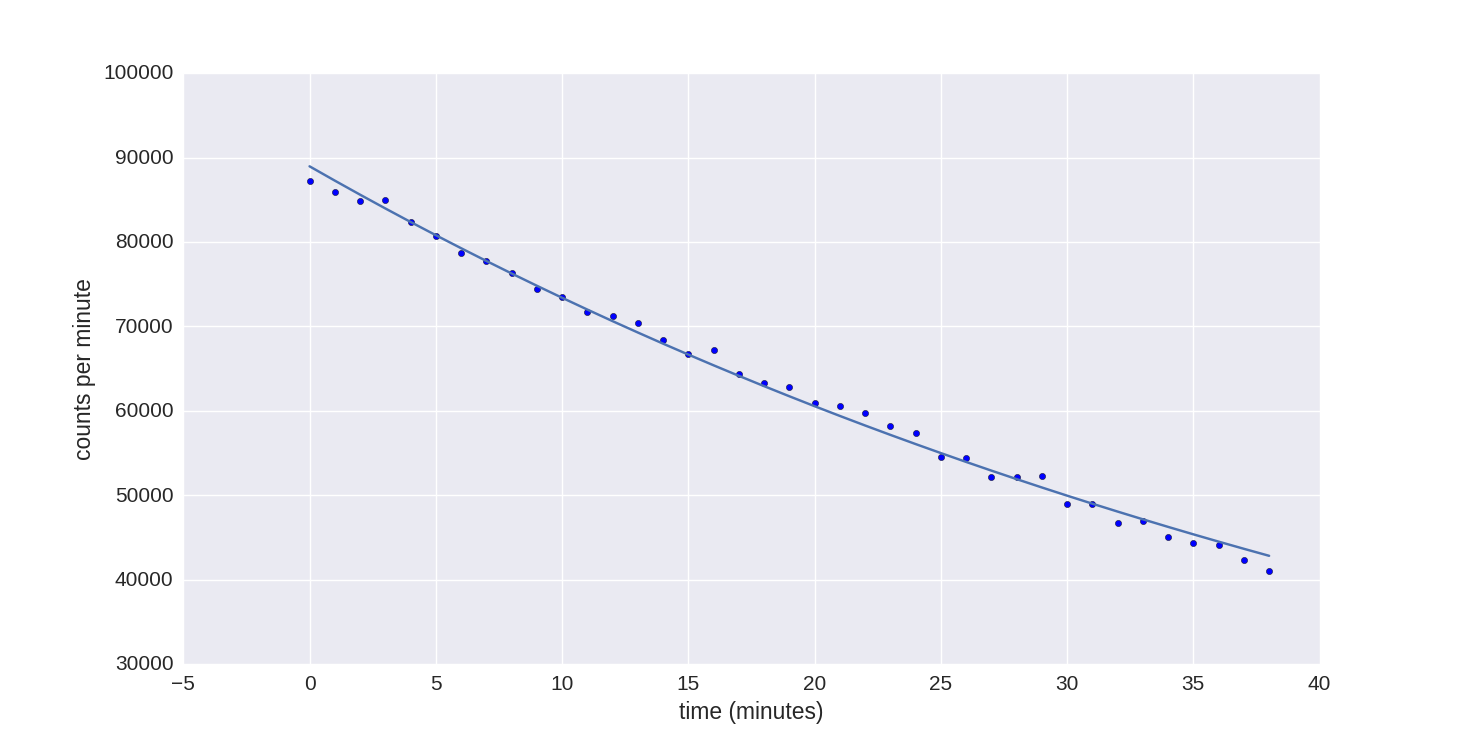
\includegraphics[height=0.4\textheight]{fig02/plot.png}
	\mycaption[Activity of the sample]{Activity of the sample.}
	\label{fig:actsample}
\end{figure}

The exponential decay of the sample follows:

\begin{equation}\label{eq9}
{A_f} = 88877.6 e^{-0.01926 t}
\end{equation}

Using the fitted value obtained for $\lambda$, equation~\ref{eq4} gives us the sample half-life $t_{1/2}$ at 35.98 minutes. This value is of no use to us in order to determine the isotopic composition of the sample.

\section{Sample emissions}

The spectrometer use was a little less straightforward. The peak analysis report is missing quite crucial information about the actual elements associated to the peaks. The results with the peaks of interests (cut off at a net peak area of 1000) are given in appendix~\ref{app:app02}. The most likely elements, based on the gamma ray peak energy and average half-life on the sample of around 36 minutes, have been selected. In this regards, for example, potential parent candidates with a half-life of less than a minute were discarded, their significant presence one hour after irradiation being ruled out. In the same vein, potential parent candidates with a half-life of more than a year were also discarded in favor of shorter lived isotopes.

Using table~\ref{tab:specdata_d}, we can try and guess the isotopic composition of the sample. One can see that if the spectrometer was correctly calibrated, the sample is likely to contain Gadolinium and Hafnium primarily, and some Tantalum, product of Hafnium disintegration.

Hafnium and Gadolinium are both neutron absorbers. Hafnium is often found in nuclear reactors control rods, while Gadolinium can be used in fresh fuel to compensate an excess of reactivity. The extensive use of those two elements in the same component is not known to the author, though the two elements have been used together in the past to build a neutron detector~\cite{imel95}.


\section{Uncertainties}

Several uncertainties sources should also be taken into account.

The measurements of the sample activity were for example not done exactly every minute, since a human action was necessary. This introduces an error on the half-life measured. Additionally, while good, an $R^2$ score of 99.5\% shows that the exponential fit is not perfect.

The spectrometer dead time was quite low, 0.6\%, but still impacts the neutron peaks. In this study, it represents 3.2 seconds of data over roughly a ten minutes recording. This can be completely discarded, it does not change the peak area and energy values. The spectrometer used is given an energy tolerance of 1 keV after energy calibration, which explains the various potential candidates presented in table~\ref{tab:specdata_p}.
